%==============================================================================
% Sjabloon onderzoeksvoorstel bachproef
%==============================================================================
% Gebaseerd op document class `hogent-article'
% zie <https://github.com/HoGentTIN/latex-hogent-article>

% Voor een voorstel in het Engels: voeg de documentclass-optie [english] toe.
% Let op: kan enkel na toestemming van de bachelorproefcoördinator!
\documentclass{hogent-article}
\usepackage[backend=biber]{biblatex}

% Invoegen bibliografiebestand
\addbibresource{voorstel.bib}

% Informatie over de opleiding, het vak en soort opdracht
\studyprogramme{Professionele bachelor toegepaste informatica}
\course{Bachelorproef}
\assignmenttype{Onderzoeksvoorstel}
% Voor een voorstel in het Engels, haal de volgende 3 regels uit commentaar
% \studyprogramme{Bachelor of applied information technology}
% \course{Bachelor thesis}
% \assignmenttype{Research proposal}

\academicyear{2023-2024} % TODO: pas het academiejaar aan

% TODO: Werktitel
\title{Evaluatie van databaseoplossingen voor e-commerce in de mode-industrie: een focus op prestaties en kosten}

% TODO: Studentnaam en emailadres invullen
\author{Yani Degrande}
\email{yani.degrande@student.hogent.be}
\projectrepo{https://github.com/Yani-Degrande/DegrandeYani-BP}

% TODO: Medestudent
% Gaat het om een bachelorproef in samenwerking met een student in een andere
% opleiding? Geef dan de naam en emailadres hier
% \author{Yasmine Alaoui (naam opleiding)}
% \email{yasmine.alaoui@student.hogent.be}

% TODO: Geef de co-promotor op
% Binnen welke specialisatierichting uit 3TI situeert dit onderzoek zich?
% Kies uit deze lijst:
%
% - Mobile \& Enterprise development
% - AI \& Data Engineering
% - Functional \& Business Analysis
% - System \& Network Administrator
% - Mainframe Expert
% - Als het onderzoek niet past binnen een van deze domeinen specifieer je deze
%   zelf
%
\specialisation{Mobile \& Enterprise development}
\keywords{Database, E-commerce, Prestaties}

\begin{document}
\emergencystretch 3em

\begin{abstract}
    Dit onderzoek richt zich op het evalueren van databasemanagementsystemen (DMBS) voor webshops
    binnen kleine tot middelgrote mode-e-commerce platformen. Hierbij wordt de focus gelegd op
    prestatie-optimalisatie en kostenbeheersing. Er zal een analyse uitgevoerd worden van de balans
    tussen de wendbaarheid van NoSQL-databases, zoals MongoDB, tegenover de bewezen stabiliteit
    van SQL-databases, zoals MySQL of PostgreSQL. De onderzoeksvraag concentreert zich op het
    identificeren van een DBMS dat uitblinkt in efficiëntie en economische haalbaarheid voor de
    beoogde gebruikersgroep. Er wordt verwacht dat de studie zal resulteren in een aanbeveling voor
    een hybride systeem dat de voordelen van beide databasetypes combineert. De methodologie omvat
    een literatuurstudie, een reeks experimenten en een vergelijkende analyse. De bedoeling van dit
    project is om bij te dragen aan een kosteneffectieve databasestrategie voor opkomende mode-e-
    commerce ondernemingen, waarbij de resultaten directe praktische implicaties zullen hebben voor
    de doelgroep.
\end{abstract}

\tableofcontents

% De hoofdtekst van het voorstel zit in een apart bestand, zodat het makkelijk
% kan opgenomen worden in de bijlagen van de bachelorproef zelf.
%---------- Inleiding ---------------------------------------------------------

\section{Introductie}%
\label{sec:introductie}

De keuze van de juiste databaseoplossing is van belang voor het succes van online mode-e-commerce platformen. Dit onderzoek is gericht op het identificeren van een databasearchitectuur die een balans biedt tussen prestaties en kostenbeheersing voor kleine tot middelgrote mode-e-commerce platformen. Gedurende een periode van vier maanden zullen verschillende databasebeheersystemen geëvalueerd worden op basis van de reactietijd, doorvoersnelheid en operationele kosten. Het einddoel van dit onderzoek is om een gestructureerde benadering te realiseren die mode-ondernemers kan helpen bij het maken van beslissingen op basis van data voor hun e-commerce systemen. De resultaten zullen een duidelijker beeld geven over hoe kleinere e-commerce ondernemingen zich kunnen schalen en klanttevredenheid kunnen verbeteren door de selectie van de gepaste technologieën. Hiermee wordt ook meteen volgende onderzoeksvraag opgelost: ``Hoe evalueren verschillende databaseoplossingen op het gebied van prestaties en kosten voor het ondersteunen van een kleine e-commerce website in de mode-industrie, binnen een onderzoeksperiode van vier maanden?''.

%---------- Stand van zaken ---------------------------------------------------

\section{Literatuurstudie}%
\label{sec:literatuurstudie}
In deze studie wordt, binnen een onderzoeksperiode van vier maanden, nagegaan welke
verschillende databaseoplossingen het meest geschikt zijn op gebied van prestaties en kosten voor
het ondersteunen van kleine e-commerce websites in de mode-industrie. Het onderzoek richt zich op
het identificeren van de meest geschikte databasesystemen die zowel efficiënt als kosteneffectief
zijn voor kleinere ondernemingen in de snel veranderende modebranche.

Voor het opbouwen van een succesvol e-commerce platform in de modebranche is het kiezen van
een concrete databaseoplossing van cruciaal belang. Tegenwoordig is het maken van die keuze
echter niet meer vanzelfsprekend. Bij het maken van een keuze moet er rekening gehouden worden
met verschillende belangrijke factoren, zoals bijvoorbeeld de kosten die deze oplossing met zich
meebrengt, de betrouwbaarheid van de database, de schaalbaarheid en de prestaties. Voor het
bouwen van een moderne e-commerce website, en meer specifiek één in de mode-industrie is er
vooral nood aan een databaseoplossing waarbij er snel en efficiënt omgegaan kan worden met grote
hoeveelheden aan ongestructureerde data en dit terwijl er een optimale gebruikerservaring
behouden wordt. Hiernaast is het ook belangrijk dat deze oplossing kosteneffectief is zodat kleine
bedrijven geen last ondervinden van te hoge operationele kosten.

De populaire NoSQL-database, MongoDB, die bekend staat voor zijn vermogen om flexibel om te
gaan met ongestructureerde data is daarom mogelijks een interessante keuze voor dynamische en
data-intensieve e-commerce platforms~\autocite{Inetum2022}. MongoDB's document-
georiënteerde benadering maakt het geschikt voor toepassingen die snelle ontwikkeling vereisen en
daarbovenop levert het goede resultaten in het omgaan met grote volumes aan diverse data. Echter,
kunnen de kosten voor het gebruik van MongoDB variëren, afhankelijk van de schaal en de vereiste
functionaliteiten, wat een aandachtspunt is voor kostengevoelige projecten.

Anderzijds is er ook de mogelijkheid om gebruik te maken van een traditionele SQL-database, zoals
MySQL of PostgreSQL. Deze databases staan bekend om hun robuustheid bij het verwerken van
gestructureerde gegevens en hun complexe zoekopdrachten. Volgens \textcite{Solarwinds} zijn traditionele databases met name geschikt voor het uitvoeren van transactie-intensieve applicaties,
zoals die vaak voorkomen in e-commerceomgevingen. Ze bieden een hoge betrouwbaarheid en sterke consistentie, maar zijn mogelijk minder flexibel in termen van schemawijzigingen. Ze kunnen ook uitdagingen opleveren bij het opschalen naar grote hoeveelheden ongestructureerde gegevens.

Naast traditionele SQL- of NoSQL-databases kan ook gebruik worden gemaakt van een Graph-database. Zowel ~\textcite{AWS} als ~\textcite{Foote2023} benadrukken dat Graph-databases een flexibeler platform bieden voor het detecteren en tot stand brengen van verbindingen en relaties. Door hun ontwerp zijn grafische databases vaak ook sneller in het presenteren van relaties dan relationele databases. Volgens ~\textcite{AWS} biedt een grafische database echter alleen meerwaarde voor datasets met sterke onderlinge verbindingen en de daarbij behorende analyses, waarbij verborgen en schijnbare relaties moeten worden onthuld.

Een mogelijke oplossing om zowel flexibel om te kunnen gaan met ongestructureerde data als
gestructureerde transactiedata is door gebruik te maken van een hybride benadering ~\autocite{DevX2023}. Dit laat toe om
gebruik te maken van een NoSQL database voor het beheer van dynamische, ongestructureerde
data, zoals MongoDB, en het gebruik van een SQL-database voor de gestructureerde transactiedata
zoals MySQL of PostgreSQL. Hierdoor zouden niet alleen de prestaties worden geoptimaliseerd maar
zouden ook de kosten beheerst kunnen worden. Dit is essentieel voor kleine bedrijven in een
competitieve markt.

Het uiteindelijke doel bestaat erin om een databaseoplossing te vinden die een optimale balans biedt
tussen de kosten en prestaties enerzijds en de flexibiliteit waarmee ingespeeld kan worden op de
veranderende behoeften van de mode-industrie anderzijds.

% Voor literatuurverwijzingen zijn er twee belangrijke commando's:
% \autocite{KEY} => (Auteur, jaartal) Gebruik dit als de naam van de auteur
%   geen onderdeel is van de zin.
% \textcite{KEY} => Auteur (jaartal)  Gebruik dit als de auteursnaam wel een
%   functie heeft in de zin (bv. ``Uit onderzoek door Doll & Hill (1954) bleek
%   ...'')



%---------- Methodologie ------------------------------------------------------
\section{Methodologie}
\label{sec:methodologie}

\subsection{Fase 1: Literatuurstudie}
\label{subsec:literatuurstudie}
In de eerste fase zal er een uitgebreide literatuurstudie uitgevoerd worden om de huidige stand van zaken in database technologieën voor e-commerce platformen in kaart te brengen. Er zullen relevante academische papers, technische documentatie, en marktanalyses bestudeerd worden. Deze fase zal tussen de drie en vier weken duren.
\textbf{Deliverables:} Een overzicht van bestaande databaseoplossingen en een samenvatting van relevante onderzoeksartikelen.

\subsection{Fase 2: Requirements-analyse}
\label{subsec:requirementsanalyse}
In de tweede fase zal er onderzocht worden wat de functionele en niet-functionele eisen zijn voor kleine tot middelgrote mode-e-commerce platformen. Dit zal gedaan worden door in gesprek te gaan of het sturen van mails met stakeholders in kleine tot middelgrote mode-e-commerce platformen. Deze fase zal ongeveer één à twee weken duren.

\textbf{Deliverables:} Een lijst van requirements voor de databasearchitectuur.

\subsection{Fase 3: Experimenteel Ontwerp}
\label{subsec:experimenteelontwerp}
In deze fase zal een reeks experimenten opgezet worden om verschillende databasebeheersystemen te evalueren. Deze experimenten zullen zich richten op prestatie-indicatoren zoals reactietijd en doorvoersnelheid. Deze fase zal ongeveer één à twee weken duren.

\textbf{Deliverables:} Een experimenteel plan en testprotocollen.

\subsection{Fase 4: Data-analyse}
\label{subsec:dataanalyse}
In fase vier zal de verzamelde data uit de experimenten geanalyseerd worden met statistische software om significante patronen en verschillen te identificeren. Deze fase zal ongeveer één à twee weken duren.

\textbf{Deliverables:} Een statistisch onderbouwd rapport met de bevindingen uit de experimenten.

\subsection{Fase 5: Vergelijkende Studie}
\label{subsec:vergelijkendestudie}
In de vijfde fase zal op basis van de data-analyse een vergelijkende studie uitgevoerd worden om de voor- en nadelen van elk databasebeheersysteem te identificeren. Deze fase zal ongeveer één tot twee weken duren.

\textbf{Deliverables:} Een gedetailleerde vergelijkingstabel en een aanbevelingsrapport.

\subsection{Fase 6: Risico-analyse}
\label{subsec:risicoanalyse}
In deze fase zal er een risico-analyse uitgevoerd worden om potentiële knelpunten en risico's in de implementatie van de aanbevolen databaseoplossingen te identificeren. Deze fase zal ongeveer een week duren.

\textbf{Deliverables:} Een risicobeoordelingsdocument.

\subsection{Fase 7: Proof of Concept (PoC)}
\label{subsec:poc}
In deze fase zal een Proof of Concept ontwikkeld worden om de haalbaarheid van de aanbevolen databasearchitectuur te demonstreren. Deze fase zal ongeveer een week duren.

\textbf{Deliverables:} Een werkend prototype en een documentatie van de ontwikkeling.

\subsection{Fase 8: Rapportering en documentatie}
\label{subsec:rapporteringendocumentatie}
Tijdens voorlaatste fase zal er een rapport en documentatie gemaakt worden van het hele proces
van het onderzoek. Dit zal gebeuren aan de hand van alle verzamelde informatie tijdens het onderzoek. Aan het einde van deze fase zal de bachelorproef volledig voltooid zijn. Deze fase zal één tot twee weken duren.

\textbf{Deliverables:} Een bijna volledig afgewerkte bachelorproef.

\subsection{Fase 9: Review en afronding}
\label{subsec:reviewenafronding}
In de laatste fase zullen alle documenten herbekeken worden om te zorgen dat alles in orde is. Deze
documenten zullen dan meerde keren gecheckt worden op taalfouten en andere fouten. Wanneer deze fase voltooid is, zal de bachelorproef klaar zijn om ingediend te worden en is het onderzoek afgelopen. Deze fase zal ongeveer één à
twee weken duren.

\textbf{Deliverables:} Een volledig afgewerkte bachelorproef.

\begin{figure}[htbp]
    \centering
    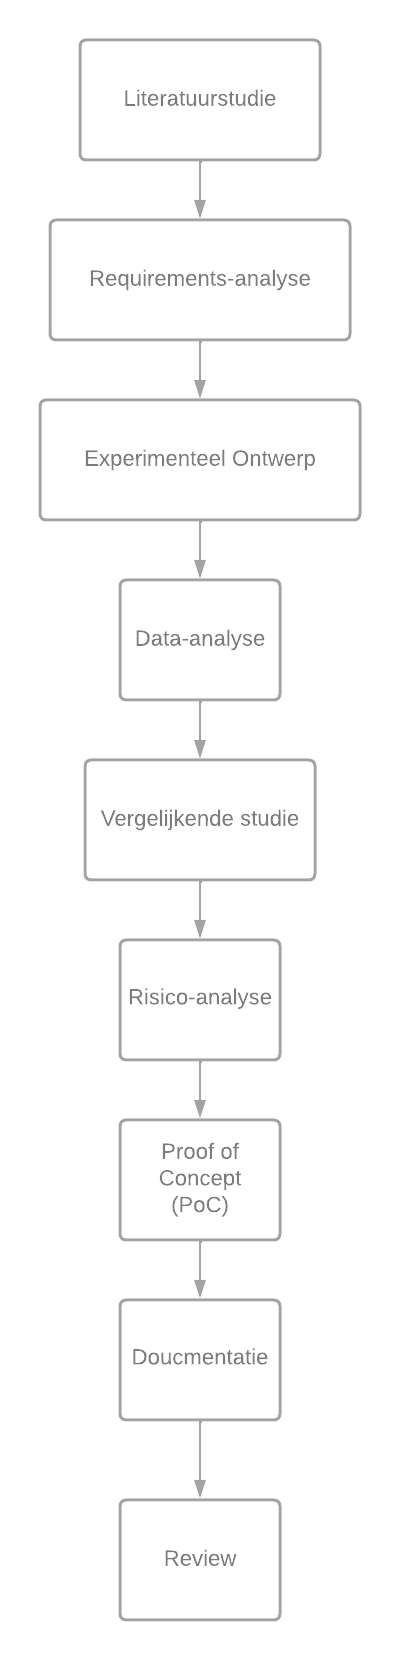
\includegraphics[width=0.3\textwidth]{Flowchart.png}
    \caption{Flowchart van het onderzoeksproces.}
    \label{fig:flowchart}
\end{figure}


%---------- Verwachte resultaten ----------------------------------------------
\section{Verwacht Resultaat en Conclusie}%
\label{sec:verwachte_resultaten}

De verworven kennis geeft momenteel aan dat de ontwikkeling van een hybride systeem, dat
MongoDB als NoSQL-database combineert met MySQL of PostgreSQL, de meest veelbelovende
benadering lijkt in termen van efficiëntie en kostenbeheersing voor kleine en middelgrote mode-e-
commerce platforms. Er wordt verwacht dat vervolgonderzoek diepere inzichten zal verschaffen die
van cruciaal belang zijn bij de keuze van het meest adequate databasemanagementsysteem. Dit
vervolgonderzoek zal de technische specificaties en operationele kostenfactoren grondig moeten
afwegen om een weloverwogen besluit te kunnen nemen.


%---------- References ----------------------------------------------



\printbibliography[heading=bibintoc]

\end{document}